\documentclass[8pt]{beamer}
\usepackage[english]{babel}

\usepackage{amsmath,amssymb,cancel}
\usepackage{graphicx}
\usepackage{multirow}
\renewcommand{\CancelColor}{\color{red}} %change cancel color to red

% vertical separator macro
\newcommand{\vsep}{
  \column{0.0\textwidth}
    
\begin{tikzpicture}
      \draw[very thick,black!10] (0,0) -- (0,7.3);
    \end{tikzpicture}
}

% More space between lines in align
% \setlength{\mathindent}{0pt}

% Beamer theme
\usetheme{UniVienna}
\usefonttheme[onlysmall]{structurebold}
\mode<presentation>
\setbeamercovered{transparent=10}

% align spacing
\setlength{\jot}{0pt}

%\setbeamertemplate{navigation symbols}{}%remove navigation symbols

\title{Seminar Tugas Akhir}
\subtitle{Pemodelan Termal Semi-empiris Satelit LAPAN-A3 \\ Menggunakan Metode Machine Learning}
\author{Ricky Sutardi 13617051}
\institute[Program Studi Teknik Dirgantara Institut Teknologi Bandung]{
  Dosen Pembimbing : \\
  Dr. Eng. Ridanto Eko Poetro ST,M.Sc. \\
  Dr. Robertus Heru Triharjanto, M.Sc. \\
  Luqman Fathurrohim ST, M.T.
}
\date{8 Agustus 2022}

\usepackage[square,numbers]{natbib}
\bibliographystyle{IEEEtranN}

\begin{document}

\renewcommand{\figurename}{Gambar}
\renewcommand{\tablename}{Tabel}

% Title
\begin{frame}
  \titlepage
\end{frame}

% Daftar Isi
\begin{frame}{Garis Besar Presentasi}
\tableofcontents
\end{frame}

% Bab 1
\section{Bab 1 - Pendahuluan}

\begin{frame}
  \frametitle{BAB I}
  \center \large PENDAHULUAN
\end{frame}

\begin{frame}
  \frametitle{Latar Belakang}
  \begin{columns}[T]
    \column{0.5\textwidth}
            \begin{block}{\center Grafik suhu \textit{multispectral imager} LAPAN-A3 sepanjang tahun 2017}
      \begin{figure}
          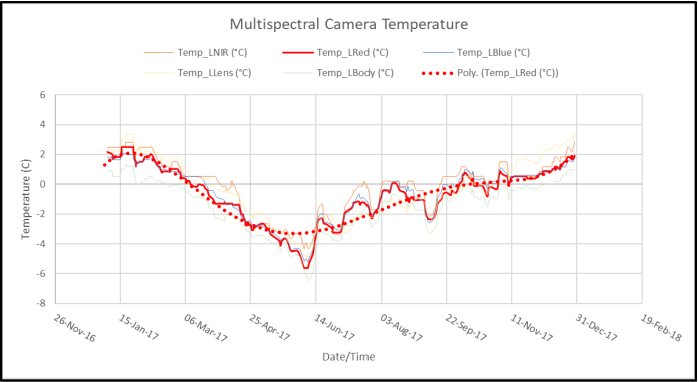
\includegraphics[width=1.0\textwidth]{figure/multispectralimager.png}
      \end{figure}
            \end{block}
    \column{0.5\textwidth}
    \begin{itemize}
        \item LAPAN-A3 adalah satelit hasil kerja sama antara Lembaga Penerbangan dan Antariksa Nasional (LAPAN) dengan Institut Pertanian Bogor (IPB) yang diluncurkan pada tahun 2016 dan memiliki misi utama observasi Bumi \cite{hasbi2013}
      \item Dari observasi data telemetri, ditemukan bahwa sistem kendali termal satelit LAPAN-A3 tidak mampu menjaga suhu \textit{payload} utama \textit{multispectral imager} di atas 0 $^\circ$C sepanjang tahun \cite{ribah2019}
      \item \textit{Multispectral imager} memiliki rentang suhu operasi 0 - 70 $^\circ$C sehingga misi pengambilan citra Bumi tidak bisa dilakukan jika suhu \textit{imager} di bawah 0 $^\circ$C
      \item Operator LAPAN harus memberikan perintah maneuver khusus untuk menaikkan suhu \textit{multispectral imager}
    \end{itemize}
  \end{columns}
\end{frame}

\begin{frame}
  \frametitle{Latar Belakang}
    \begin{itemize}
      \item Dibutuhkan sebuah model termal sederhana yang dapat memprediksi suhu sisi-sisi satelit agar permasalahan tidak terulang pada desain satelit LAPAN selanjutnya
      \item Pemodelan termal satelit konvensional membutuhkan perhitungan numerik yang kompleks \cite{das} atau perangkat lunak komersial khusus \cite{boudjemai2015}
      \item Metode \textit{machine learning} sudah umum digunakan dalam analisis termal satelit karena dapat mengurangi kompleksitas dan jumlah perhitungan dalam pemodelan termal satelit \cite{junior2017}\cite{escobar2016}\cite{xiong2020}
      \item Akan dibuat sebuah model termal semi-empiris menggunakan metode regresi linear \textit{machine learning} yang dapat memprediksi perubahan suhu sisi-sisi satelit LAPAN-A3
      \item Model termal tersebut akan dilatih, diuji, dan dievaluasi berdasarkan data telemetri aktual satelit LAPAN-A3 pada periode observasi 19 dan 20 Mei 2018
    \end{itemize}
\end{frame}


\begin{frame}
  \frametitle{Rumusan Masalah}
  \begin{enumerate}
    \item Bagaimana pemodelan termal semi-empiris satelit LAPAN-A3 menggunakan metode \textit{machine learning} dapat dilakukan?
    \item Bagaimana perbandingan perubahan suhu sisi-sisi satelit hasil prediksi model termal satelit dengan data telemetri satelit?
    \item Bagaimana performa model termal satelit yang dihasilkan?
  \end{enumerate}
\end{frame}

\begin{frame}
  \frametitle{Tujuan Penelitian}
  \begin{enumerate}
    \item Melakukan penjabaran langkah-langkah untuk membuat model termal satelit \textit{node} banyak secara semi-empiris menggunakan metode \textit{machine learning}
    \item Membuat model termal satelit yang dapat memprediksi perubahan suhu sisi-sisi satelit LAPAN-A3
    \item Membandingkan perubahan suhu \textit{node} satelit hasil prediksi model termal dengan data telemetri satelit
    \item Menganalisis performa hasil prediksi dari model termal satelit yang telah dibuat
\end{enumerate}

\end{frame}

\begin{frame}
  \frametitle{Batasan Penelitian}
  \begin{enumerate}
    \item Pemodelan termal satelit LAPAN-A3 dilakukan untuk periode observasi 19 dan 20 Mei 2018
    \item Selama periode observasi, satelit dianggap tidak mengalami perubahan massa dan karakteristik termal
    \item Satelit LAPAN-A3 dianggap berbentuk balok dan dibagi menjadi 7
	\textit{node} mewakili 6 sisi satelit dan plat tengah satelit dengan aturan
		konversi sumbu menjadi nomor \textit{node} sebagai berikut : X+ = 1, X- =
		2, Y+ = 3, Y- = 4, Z+ = 5, Z- = 6, serta plat tengah = 7
  \end{enumerate}
\end{frame}

\begin{frame}
  \frametitle{Metodologi}
  \begin{columns}[T]
    \column{0.39\textwidth}
    \begin{block}{\center Metodologi penelitian}
      \begin{center}
    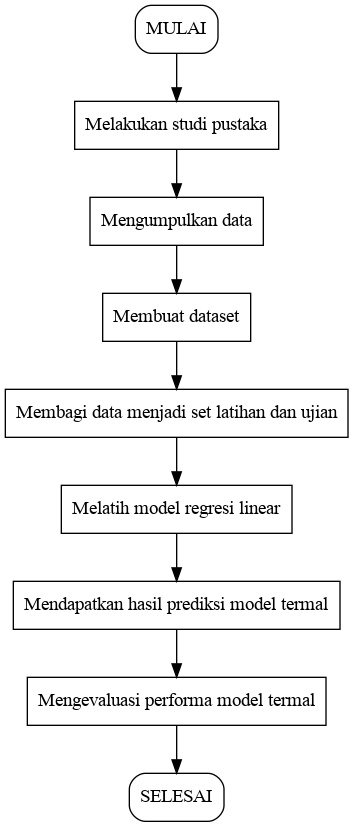
\includegraphics[width=0.5\textwidth]{figure/graph_metodologi.png}
      \end{center}
    \end{block}
    \column{0.02\textwidth}
    \column{0.59\textwidth}
    \begin{block}{\center Algoritma pembuatan dataset}
      \begin{center}
    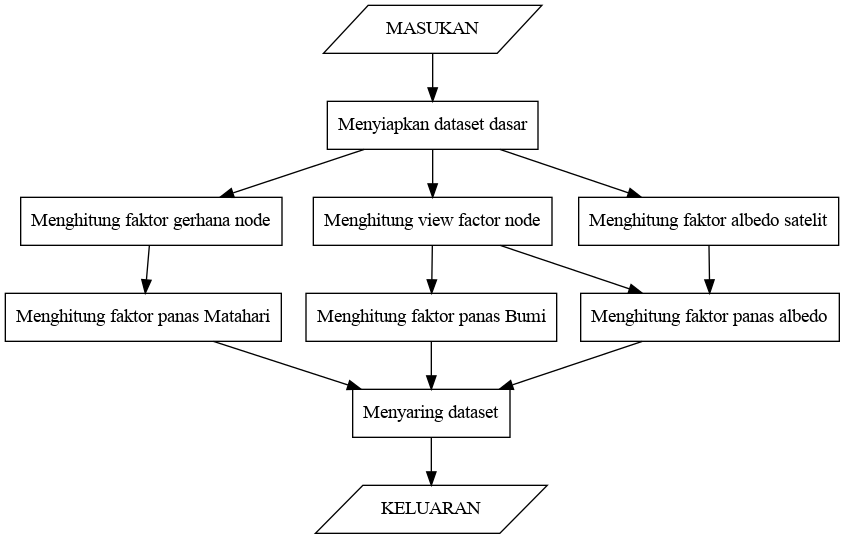
\includegraphics[width=1.0\textwidth]{figure/graph_algoritma.png}
      \end{center}
    \end{block}
    Kode sumber pemrograman karya tulis dapat diakses di https://github.com/sutricky/a3thermalmodel
  \end{columns}
  
\end{frame}

\begin{frame}
  \frametitle{Sistematika Penulisan}
\begin{enumerate}
\item Bab 1 Pendahuluan

Bab ini membahas latar belakang, rumusan masalah, tujuan penelitian, batasan
penelitian, metodologi karya tulis, dan sistematika penulisan.

\item Bab 2 Tinjauan Pustaka

Bab ini membahas dasar teori yang digunakan dalam rangka pengerjaan karya tulis ini.

\item Bab 3 Pembuatan Model Termal Satelit LAPAN-A3

Bab ini menjabarkan langkah-langkah untuk membuat model termal semi-empiris
		satelit LAPAN-A3 dengan menggunakan metode \textit{machine learning}.

\item Bab 4 Hasil dan Analisis

Bab ini berisi hasil prediksi suhu sisi-sisi satelit LAPAN-A3 serta analisis performa model termal satelit LAPAN-A3 yang dihasilkan dari bab sebelumnya.

\item Bab 5 Kesimpulan dan Saran

Bab ini berisi kesimpulan dari penelitian yang telah dilakukan dan saran
untuk penelitian selanjutnya.
\end{enumerate}
\end{frame}


% Bab 2
\section{Bab 2 - Tinjauan Pustaka}
\begin{frame}
  \frametitle{BAB II}
  \center \large TINJAUAN PUSTAKA
\end{frame}
\begin{frame}
  \frametitle{Satelit LAPAN-A3}
  \begin{columns}[T]
    \column{0.4\textwidth}
      \begin{block}{\center Desain LAPAN-A3}
      \begin{figure}
          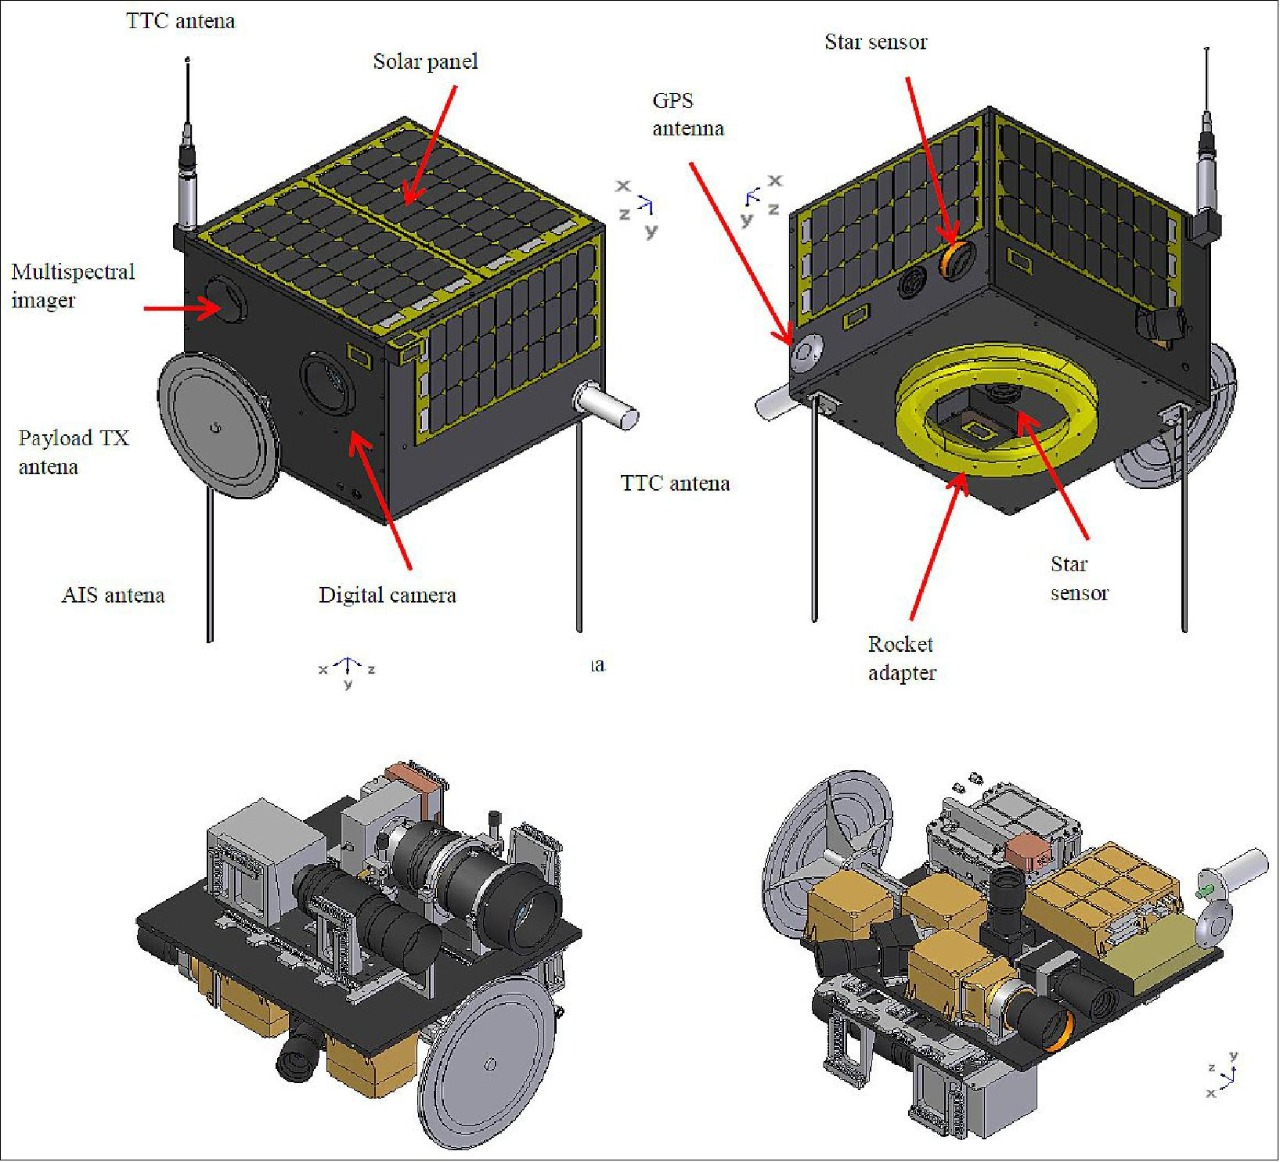
\includegraphics[width=0.9\textwidth]{figure/a3overview.jpg}
      \end{figure}
      \end{block}
    \column{0.6\textwidth}
      \begin{itemize}
        \item Satelit ke-3 dengan sistem kendali termal pasif (tidak menggunakan daya) yang dikembangkan LAPAN setelah LAPAN-A1 dan LAPAN-A2
        \item Memiliki misi utama berupa observasi Bumi untuk mendukung ketahanan pangan Indonesia
        \item Membawa 4 \textit{payload} : \textit{multispectral imager}, \textit{digital space camera}, \textit{automatic identification system}, dan \textit{experimental thermal imager} \cite{hartono2019}
        \item Memiliki orbit lingkaran \textit{sun-synchronous} dengan ketinggian 515 km dan inklinasi $97.5^\circ$
        \item Menggunakan 5 panel surya yang tersebar di 4 sisi satelit sebagai sumber energi
        \item Ke-enam sisi satelit dilengkapi sensor untuk mendeteksi arah sinar Matahari
      \end{itemize}
  \end{columns}
\end{frame}

\begin{frame}
  \frametitle{Two-line Element}
  \begin{columns}[c]
    \column{0.3\textwidth}
      \begin{itemize}
        \item Format data untuk mendeskripsikan parameter orbit objek ruang angkasa
        \item Dirilis ke publik secara berkala oleh \textit{United States Space Command} (USSPACECOM)
        \item Digunakan untuk mensimulasikan orbit satelit sehingga vektor posisi dan kecepatan satelit pada suatu waktu dapat dihitung
      \end{itemize}

    \column{0.7\textwidth}
          \begin{block}{\center Penjelasan baris dan kolom TLE}
      \begin{figure}
          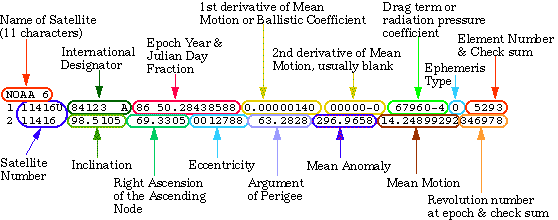
\includegraphics[width=0.8\textwidth]{figure/tlemeaning.png}
      \end{figure}
          \end{block}
  \end{columns}
\end{frame}

\begin{frame}
  \frametitle{Pemodelan Termal Satelit}
  \begin{columns}[T]
    \column{0.45\textwidth}
    \begin{block}{\center Sumber perpindahan panas satelit}
      \begin{itemize}
        \item Internal : konduksi, konveksi, dan radiasi antar komponen satelit
        \item Eksternal : radiasi dari Matahari, radiasi dari Bumi, albedo dari Bumi, dan radiasi ke ruang angkasa
      \end{itemize}
      \begin{figure}
        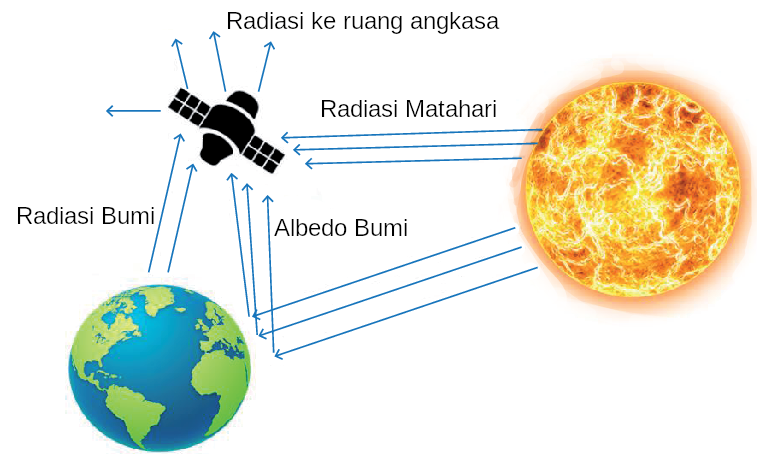
\includegraphics[width=1.0\textwidth]{figure/external_source.png}
        Sumber perpindahan panas eksternal satelit yang mengorbit Bumi \cite{abdelkhalek2019}
      \end{figure}
    \end{block}
    \column{0.55\textwidth}
    \begin{itemize}
      \item Pemodelan termal satelit bertujuan untuk memodelkan karakteristik termal satelit lewat analisis perpindahan panas satelit
      \item Metode semi-empiris berarti menggunakan asumsi, pendekatan, dan generalisasi untuk menyederhanakan perhitungan teoretis sesuai hasil observasi pada satelit
      \item Satelit dimodelkan menjadi titik-titik analisis diskrit (\textit{node}) yang diasumsikan memiliki suhu dan karakteristik termal yang sama
      \item Persamaan keseimbangan termal satelit dapat dilinearisasi menjadi persamaan laju perubahan suhu \textit{node} satelit
      \item Persamaan laju perubahan suhu \textit{node} satelit diselesaikan menggunakan metode regresi linear \textit{machine learning}
    \end{itemize}
  \end{columns}
\end{frame}

\begin{frame}
  \frametitle{Pemodelan Termal Satelit}
  \begin{columns}[T]
    \column{0.49\textwidth}
    \begin{block}{\normalsize Persamaan termal satelit LAPAN-A3}
      \small
  Persamaan laju perubahan suhu \textit{node i} pada model satelit LAPAN-A3 dengan $N$ node yang sudah memperhitungkan sumber-sumber perpindahan panas dan interaksi dengan \textit{node-node} lain $j$ \cite{martinez2022}:
\begin{equation}
\label{eq:lineq}
\begin{split}
	\frac{\Delta T_i}{\Delta t} = &\ \frac{c_S}{C_i I_0} I_{i}(t) F_{e,i}(t) \\
	&+ \frac{c_a}{C_i} F_{i,E}(t) F_a(t) \\
	&+ \frac{c_E}{C_i} F_{i,E}(t) T_{i}(t)^4 \\
	&- \frac{\left( \mathop{\sum_{j=1}^{N}}_{j \neq i} \sigma R_{ij} + c_{env} \right) }{C_i} T_{i}(t)^4 \\
	&+ \mathop{\sum_{j=1}^{N}}_{j \neq i} \frac{G_{ij}}{C_i} \left(T_j(t) - T_i(t)\right) \\
	&+ \mathop{\sum_{j=1}^{N}}_{j \neq i} \frac{\sigma R_{ij}}{C_i}T_{j}(t)^4 \\
	&+ \frac{\dot{Q}_{dis,i}}{C_i}
\end{split}
\end{equation}
    \end{block}
    \column{0.51\textwidth}
      \begin{center}Keterangan\end{center}
      \begin{description}
          \tiny
        \item[$\Delta T_{i}$] Perubahan suhu \textit{node i}
        \item[$\Delta t_{i}$] Selang waktu
        \item[$C_{i}$] Kapasitas termal \textit{node i}
        \item[$c_S$] Koefisien suku panas akibat Matahari
        \item[$I_{i}$] Arus sensor Matahari \textit{node i}
        \item[$I_{0}$] Arus maksimum sensor Matahari satelit
        \item[$F_{e,i}$] Faktor gerhana \textit{node i}
        \item[$c_{a}$] Koefisien suku panas akibat albedo
        \item[$F_{i,E}$] Nilai \textit{view factor} dari \textit{node i} ke Bumi
        \item[$F_{a}$] Faktor albedo satelit 
        \item[$c_{E}$] Koefisien suku panas akibat Bumi
        \item[$T_{i}, T_{j}$] Suhu \textit{node}
        \item[$\sigma$] Konstanta Stefan-Boltzmann 
        \item[$R_{ij}$] Koefisien kopling radiasi antara \textit{node i} dan \textit{node j}
        \item[$c_{env}$] Koefisien suku disipasi ke lingkungan ruang angkasa
        \item[$G_{ij}$] Koefisien kopling konduksi antara \textit{node i} dan \textit{node j}
        \item[$\dot{Q}_{dis,i}$] Laju masukan panas akibat disipasi elektrik \textit{node i}

\end{description}
  \end{columns}
\end{frame}

\begin{frame}
  \frametitle{Pemodelan Termal Satelit}
  \begin{columns}[T]
    \column{0.39\textwidth}
    \begin{itemize}
      \item Pemodelan termal konvensional mengharuskan perhitungan semua variabel pada ruas kanan persamaan laju perubahan suhu \textit{node} (Persamaan (\ref{eq:lineq}))
      \item Dengan metode regresi linear \textit{machine learning}, variabel yang masih harus dicari hanya variabel-variabel yang berubah terhadap waktu (ditandai (t) pada Persamaan (\ref{eq:lineq})) atau hasil perkaliannya
    \end{itemize}
    \column{0.01\textwidth}
    \column{0.59\textwidth}
    \begin{block}{\center Variabel yang masih belum diketahui}
    \begin{table}[H]
\begin{center}
\begin{tabular}{|l|l|}
\hline
Variabel & Deskripsi \\ \hline
	$I_i F_{e,i}$        & Faktor panas akibat Matahari         \\ \hline
	$F_{i,E} F_a$        & Faktor panas akibat albedo         \\ \hline
	$F_{i,E} T_i^4$        & Faktor panas akibat Bumi         \\ \hline
	$T_i, T_j, T_i^4,$ dan $T_j^4$        & Suhu \textit{node-node} satelit         \\ \hline
\end{tabular}
\end{center}
\end{table}
    \end{block}
    \column{0.01\textwidth}
  \end{columns}
\end{frame}

\begin{frame}
  \frametitle{Pemodelan Termal Satelit}
  \begin{columns}[T]
    \column{0.49\textwidth}
    \begin{block}{\center \normalsize Faktor gerhana \textit{node} satelit $F_{e,i}$}
      Bernilai 1 jika \textit{node} menerima sinar Matahari dan 0 jika \textit{node} tidak menerima sinar Matahari
    \end{block}
    \begin{block}{\center \normalsize Faktor albedo satelit $F_a$}
      \begin{equation}
\label{eq:albedofactor}
F_a = \left( \frac{1 + \cos{\phi}}{2} \right)^2 \left[ 1 - \left( \frac{\phi}{\phi_{es}} \right)^2 \right] F_e
\end{equation}
    \end{block}
    \center Keterangan
    \small
      \begin{description}
        \item[$F_a$] Faktor albedo satelit
        \item[$\phi$] Posisi sudut satelit
        \item[$\phi_{es}$] Posisi sudut satelit saat memasuki fase gerhana
        \item[$F_e$] Faktor gerhana satelit; bernilai 0 jika satelit dalam fase gerhana dan 1 jika tidak dalam fase gerhana

\end{description}
    \column{0.02\textwidth}
    \column{0.49\textwidth}
    \begin{block}{\center \normalsize \textit{View factor node} satelit ke Bumi $F_{i,E}$}
      \begin{itemize}
        \item Nilai \textit{view factor} merupakan proporsi radiasi dari suatu permukaan yang diterima oleh permukaan lain
        \item Satelit diasumsikan berbentuk balok dan jauh lebih kecil dibandingkan Bumi
        \item Nilai \textit{view factor node} satelit ke Bumi didekati dengan \textit{view factor} plat persegi panjang ke bola
      \end{itemize}
    \end{block}
  \end{columns}
\end{frame}


\begin{frame}
  \frametitle{Machine Learning}
  \begin{columns}[c]
    \column{0.49\textwidth}
    \begin{block}{\center Cara kerja metode \textit{machine learning}}
      \begin{figure}
        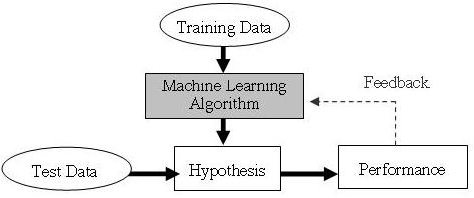
\includegraphics[width=0.8\textwidth]{figure/mldiagram.jpg}
      \end{figure}
      \begin{enumerate}
        \item Dataset masukan dibagi menjadi set latihan dan ujian
        \item Set latihan dijadikan data masukan algoritma \textit{machine learning}
        \item Algoritma \textit{machine learning} akan membuat hipotesis berupa model yang menjelaskan hubungan antar data masukan
        \item Hipotesis diterapkan pada set ujian
        \item Performa model dievaluasi dan dijadikan umpan balik
      \end{enumerate}
    \end{block}
    \column{0.02\textwidth}
    \column{0.49\textwidth}
    \begin{itemize}
      \item Bidang yang mempelajari metode dan algoritma komputer yang dapat
        menggunakan data untuk meningkatkan performa dalam mengerjakan
        serangkaian tugas secara otomatis \cite{mitchell1997}
      \item Algoritma \textit{machine learning} mampu mempelajari sendiri karakteristik permasalahan yang harus diselesaikan dari kumpulan data yang diberikan
      \item Metode \textit{machine learning} umum digunakan pada permasalahan yang melibatkan data dalam jumlah banyak seperti pengelompokkan wajah manusia, pembuatan rekomendasi produk, dan analisis finansial modern
    \end{itemize}
  \end{columns}
\end{frame}

\begin{frame}
  \frametitle{Machine Learning}
  \begin{columns}[T]
    \column{0.49\textwidth}
    \begin{block}{\center Aplikasi \textit{machine learning} dalam pemodelan termal satelit}
      \begin{itemize}
        \item Metode \textit{machine learning} digunakan untuk membuat model regresi linear persamaan termal satelit LAPAN-A3
        \item Model \textit{machine learning} dilatih dengan data masukan parameter satelit dan data keluaran laju perubahan suhu \textit{node}
        \item Algoritma \textit{machine learning} akan mencari koefisien suku-suku persamaan laju perubahan suhu \textit{node} yang dapat memetakan data masukan ke data keluaran
        \item Model termal yang dihasilkan kemudian digunakan untuk memprediksi suhu \textit{node-node} satelit
      \end{itemize}
    \end{block}
    \column{0.02\textwidth}
    \column{0.49\textwidth}
    \begin{block}{\center Evaluasi performa model \\ \textit{machine learning}}
      \begin{enumerate}
        \item Skor koefisien determinasi ($R^2$) \cite{gupta2021}
          \begin{itemize}
            \item Mengukur akurasi model dalam memprediksi tren data observasi
            \item Bernilai maksimum 1
            \item Semakin tinggi, semakin dekat tren hasil prediksi model dengan data observasi
            \item Menunjukkan proporsi variasi nilai data observasi yang dapat diprediksi model
          \end{itemize}
        \item Nilai \textit{root mean-square error} (RMSE) \cite{zheng}
          \begin{itemize}
            \item Mengukur akurasi model dalam memprediksi nilai data observasi
            \item Selalu bernilai positif
            \item Semakin rendah, semakin dekat hasil prediksi model dengan nilai data observasi
            \item Bergantung pada skala dan jumlah dataset model
          \end{itemize}
        \end{enumerate}
    \end{block}
  \end{columns}
\end{frame}

\begin{frame}
  \frametitle{Perangkat Lunak}
  \begin{columns}[c]
    \column{0.5\textwidth}
  Pemrograman dilakukan dalam bahasa Python dan modul yang digunakan adalah sebagai berikut :
  \begin{enumerate}
    \item Pandas
    \item Numpy
    \item Matplotlib
    \item Scikit-learn
    \item Skyfield
    \item Scipy
  \end{enumerate}
    \column{0.5\textwidth}
         
\includegraphics[width=0.3\textwidth]{figure/pandas.png}
         
\includegraphics[width=0.3\textwidth]{figure/numpy.png}
         
\includegraphics[width=0.3\textwidth]{figure/matplotlib.png}
         
\includegraphics[width=0.3\textwidth]{figure/scikit.png}
         
\includegraphics[width=0.3\textwidth]{figure/skyfield.png}
         
\includegraphics[width=0.2\textwidth]{figure/scipy.png}
  \end{columns}
\end{frame}


% Bab 3
\section{Bab 3 - Pembuatan Model Termal Satelit LAPAN-A3}
\begin{frame}
  \frametitle{BAB III}
  \center \large PEMBUATAN MODEL TERMAL SATELIT LAPAN-A3
\end{frame}
\begin{frame}
  \frametitle{Pengumpulan Data}
  Data yang dikumpulkan berupa data telemetri aktual LAPAN-A3 dan data TLE. Data telemetri dikumpulkan dari data internal LAPAN dan data TLE dkumpulkan dari situs Celestrak.
  \begin{block}{\center Contoh data telemetri satelit LAPAN-A3}
      \begin{figure}
          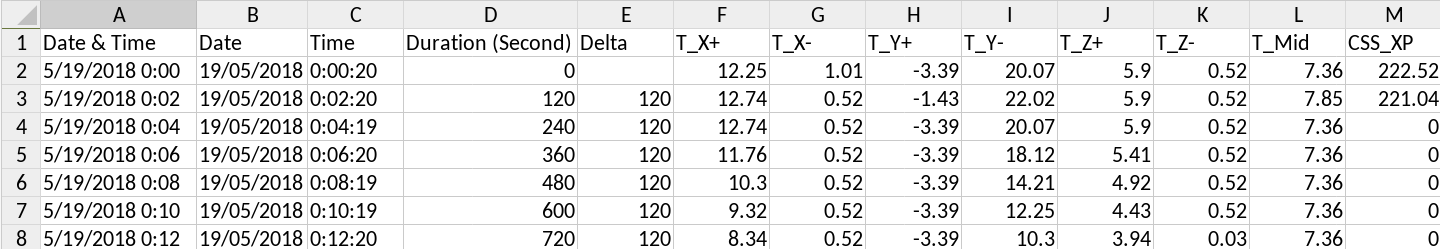
\includegraphics[width=0.8\textwidth]{figure/telea3.png}
      \end{figure}
    \end{block}
    \begin{block}{\center Contoh data TLE satelit LAPAN-A3}
      \begin{figure}
          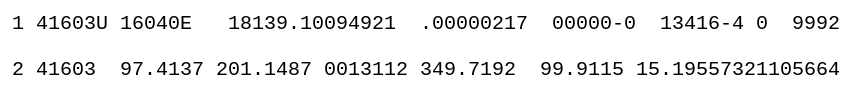
\includegraphics[width=0.5\textwidth]{figure/tlea3.png}
      \end{figure}
    \end{block}
\end{frame}

\begin{frame}
  \frametitle{Pembuatan Dataset}
  \begin{columns}[T]
    \column{0.49\textwidth}
    \begin{block}{\center 1. Persiapan dataset dasar}
      Mengubah data mentah yang sudah dikumpulkan (data telemetri dan TLE) menjadi bentuk dan satuan yang dibutuhkan :
      \begin{itemize}
        \item Suhu \textit{node} satelit dalam satuan K
        \item Arus sensor Matahari dalam satuan A
        \item Sudut sikap satelit dalam satuan rad
        \item Data waktu satelit dipisah menjadi format tahun, bulan, tanggal, jam, menit, dan detik
      \end{itemize}
    \end{block}
    \column{0.02\textwidth}
    \column{0.49\textwidth}
    \begin{block}{\center 2. Perhitungan faktor termal satelit}
      Menghitung variabel-variabel yang dibutuhkan untuk menyelesaikan persamaan laju perubahan suhu \textit{node} :
      \begin{enumerate}
        \item Faktor panas akibat Matahari
        \item Faktor panas akibat albedo
        \item Faktor panas akibat Bumi
      \end{enumerate}
    \end{block}
  \end{columns}
\end{frame}

\begin{frame}
  \frametitle{Pembuatan Dataset}
  \begin{columns}[T]
    \column{0.49\textwidth}
      \begin{block}{\center 3. Penyaringan dataset}
        Menghilangkan kesalahan dan \textit{outlier} bacaan sensor yang dapat mengurangi akurasi model termal.
      Kriteria penyaringan dataset :
\begin{enumerate}
\item Selang waktu antar pengamatan maksimal 120 s 
\item Skor standar suhu \textit{node} satelit memiliki rentang -3 sampai dengan 3
\item Skor standar laju perubahan suhu \textit{node} satelit berkisar dari -3 sampai dengan 3 
\end{enumerate}
      \end{block}
    \column{0.02\textwidth}
    \column{0.49\textwidth}
      \begin{block}{\center Skor standar}
\begin{equation}
\label{eq:zscore}
\small
	z = \frac{x - \mu}{\sigma}
\end{equation}
      \end{block}
      \small
\center Keterangan \cite{massaron}

    \begin{description}
        \item[$z$] Skor standar data
        \item[$x$] Nilai data
        \item[$\mu$] Rata-rata dataset
        \item[$\sigma$] Standar deviasi dataset
    \end{description}

  \end{columns}
\end{frame}

\begin{frame}
  \frametitle{Pelatihan dan Pengujian Model}
  \begin{columns}[T]
    \column{0.39\textwidth}
      \begin{itemize}
        \item Dataset yang sudah disaring dibagi menjadi set latihan dan ujian dengan proporsi 0.7:0.3 untuk menghindari \textit{overfitting} dan \textit{underfitting}
        \item Set latihan digunakan untuk melatih model menghitung koefisien persamaan laju perubahan suhu \textit{node}
        \item Set ujian digunakan untuk menghasilkan prediksi suhu \textit{node} satelit
      \end{itemize}
    \column{0.02\textwidth}
    \column{0.59\textwidth}
          \begin{block}{\center Detail jumlah dataset model \textit{machine learning}}
      \begin{table}[H]
        \begin{center}
          \label{table:dataset}
          \begin{tabular}{|c|cc|}
            \hline
            \multirow{2}{*}{Tanggal} & \multicolumn{2}{c|}{Dataset}                 \\ \cline{2-3} 
             & \multicolumn{1}{c|}{Set latihan} & Set ujian \\ \hline
            19 Mei 2018              & \multicolumn{1}{c|}{201}         & 87        \\ \hline
            20 Mei 2018              & \multicolumn{1}{c|}{180}         & 78        \\ \hline
          \end{tabular}
        \end{center}
      \end{table}
          \end{block}
    \begin{block}{\center \normalsize Overfitting}
      \small
    Fenomena berkurangnya akurasi model dalam memprediksi dataset baru akibat
    terlalu fokus dengan dataset masukan.
    \end{block}
    \begin{block}{\center \normalsize Underfitting}
      \small
      Ketidakmampuan model dalam menangkap tren atau fitur dataset masukan
      sehingga tidak dapat memprediksi nilai data dengan tepat.
    \end{block}
  \end{columns}
\end{frame}


% Bab 4
\section{Bab 4 - Hasil dan Analisis}
\begin{frame}
  \frametitle{BAB IV}
  \center \large HASIL DAN ANALISIS
\end{frame}
\begin{frame}
  \frametitle{Hasil Pemodelan Termal Satelit LAPAN-A3}
  \center Grafik suhu \textit{node} satelit vs waktu 19 Mei 2018
  \begin{columns}[T]
    \column{0.5\textwidth}
      \begin{figure}
          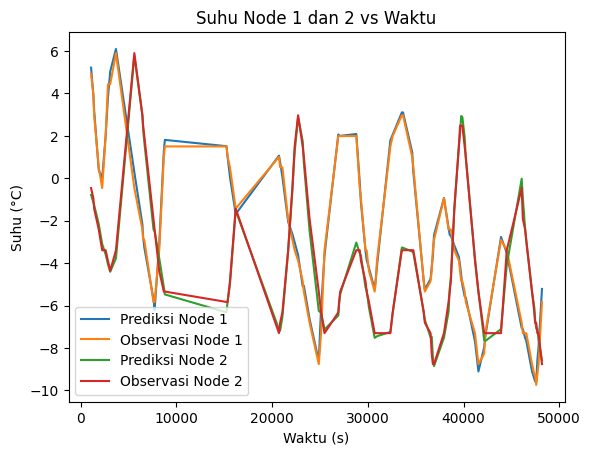
\includegraphics[width=0.7\textwidth]{figure/paper_node12_temp_2018-05-19.png}
      \end{figure}
      \begin{figure}
          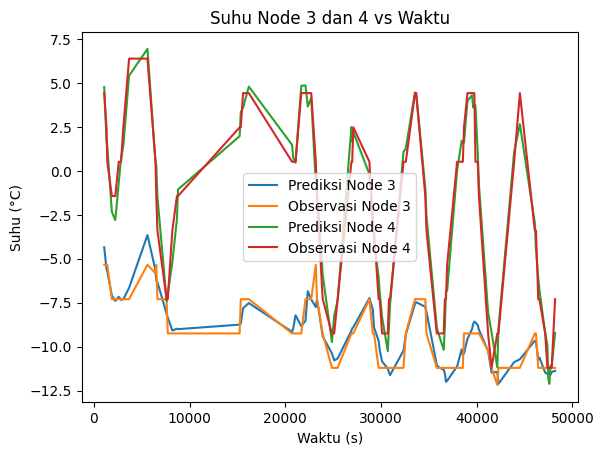
\includegraphics[width=0.7\textwidth]{figure/paper_node34_temp_2018-05-19.png}
      \end{figure}
    \column{0.5\textwidth}
      \begin{figure}
          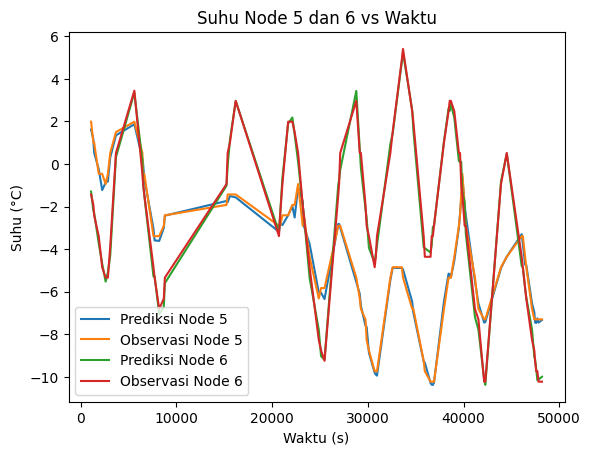
\includegraphics[width=0.7\textwidth]{figure/paper_node56_temp_2018-05-19.png}
      \end{figure}
      \begin{figure}
          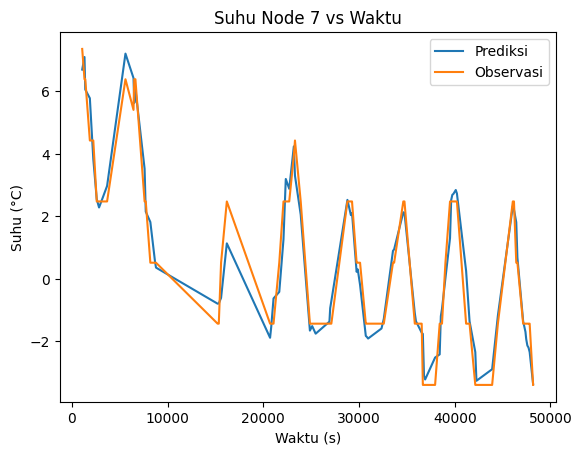
\includegraphics[width=0.7\textwidth]{figure/paper_node7_temp_2018-05-19.png}
      \end{figure}
  \end{columns}
\end{frame}

\begin{frame}
  \frametitle{Hasil Pemodelan Termal Satelit LAPAN-A3}
  \center Grafik suhu \textit{node} satelit vs waktu 20 Mei 2018
  \begin{columns}[T]
    \column{0.5\textwidth}
      \begin{figure}
          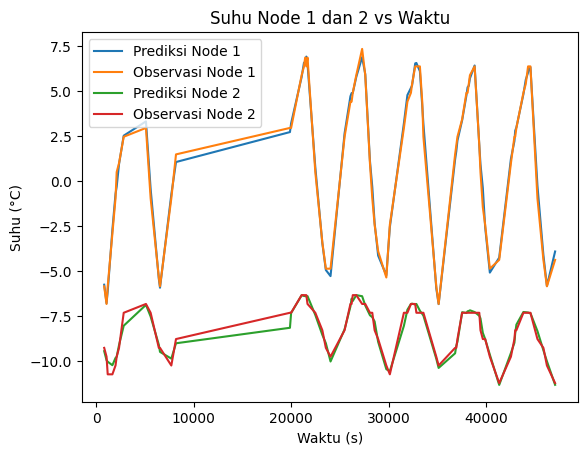
\includegraphics[width=0.7\textwidth]{figure/paper_node12_temp_2018-05-20.png}
      \end{figure}
      \begin{figure}
          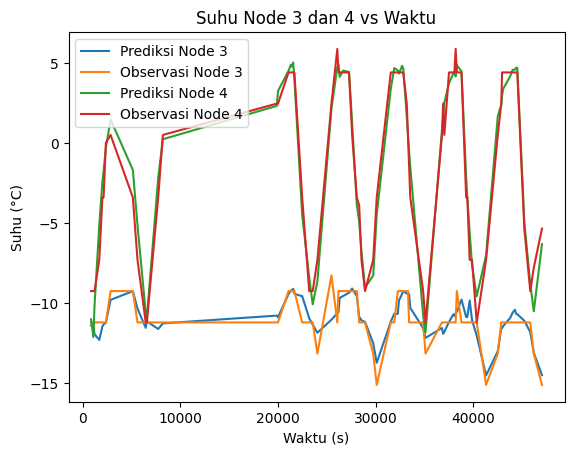
\includegraphics[width=0.7\textwidth]{figure/paper_node34_temp_2018-05-20.png}
      \end{figure}
    \column{0.5\textwidth}
      \begin{figure}
          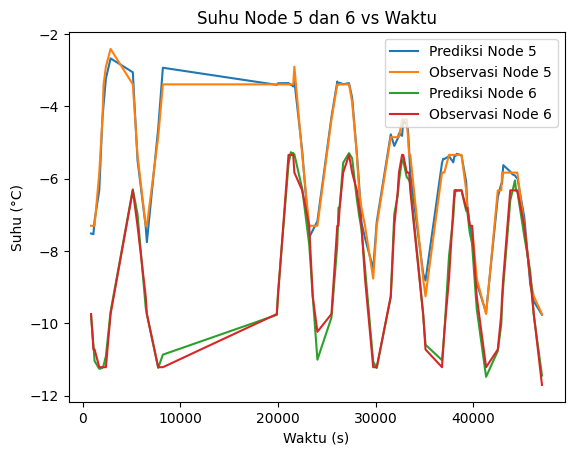
\includegraphics[width=0.7\textwidth]{figure/paper_node56_temp_2018-05-20.png}
      \end{figure}
      \begin{figure}
          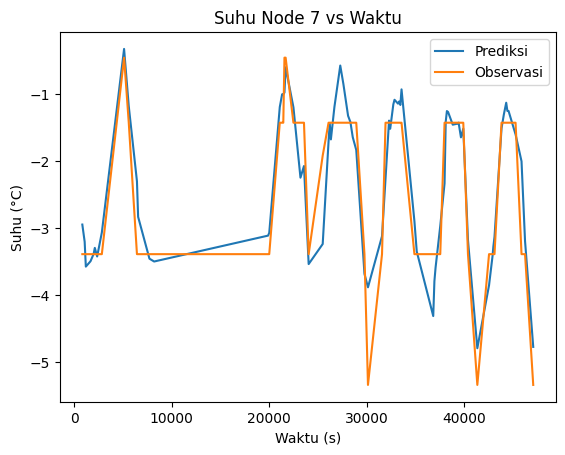
\includegraphics[width=0.7\textwidth]{figure/paper_node7_temp_2018-05-20.png}
      \end{figure}
  \end{columns}
\end{frame}


\begin{frame}
  \frametitle{Hasil Pemodelan Termal Satelit LAPAN-A3}
  \begin{columns}[T]
    \column{0.5\textwidth}
    \center 19 Mei 2018
      \begin{figure}
          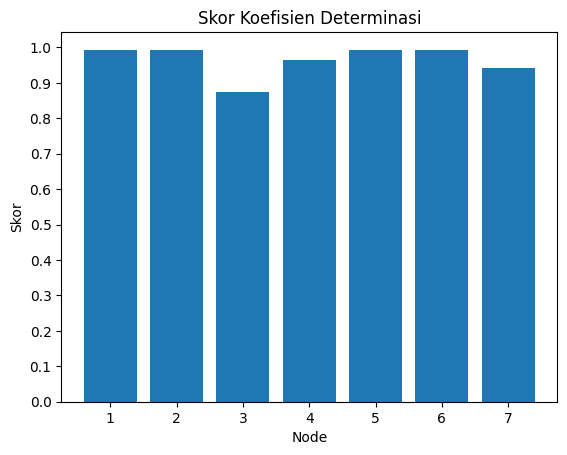
\includegraphics[width=0.6\textwidth]{figure/r2_2018-05-19.png}
      \end{figure}
      \begin{figure}
          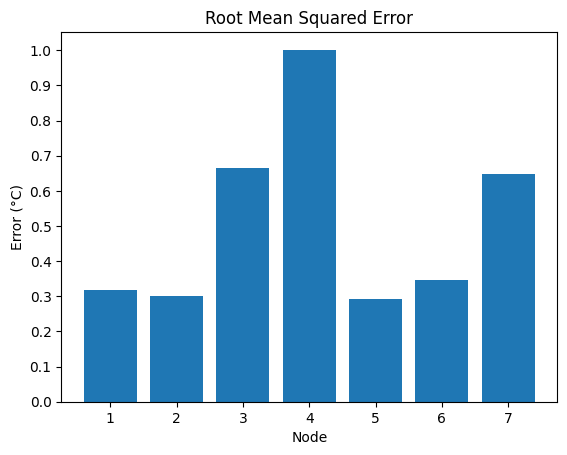
\includegraphics[width=0.6\textwidth]{figure/rmse_2018-05-19.png}
      \end{figure}
    \column{0.5\textwidth}
    \center 20 Mei 2018
      \begin{figure}
          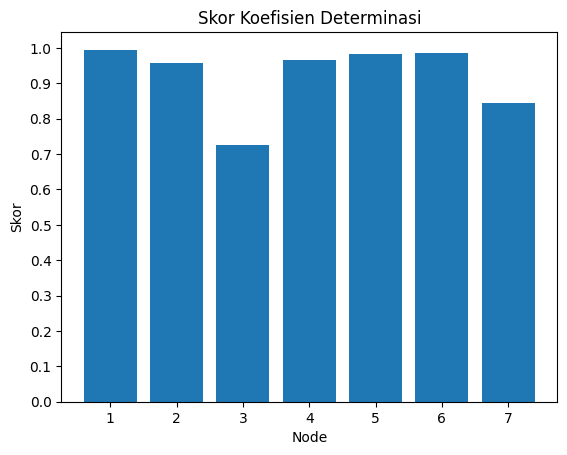
\includegraphics[width=0.6\textwidth]{figure/r2_2018-05-20.png}
      \end{figure}
      \begin{figure}
          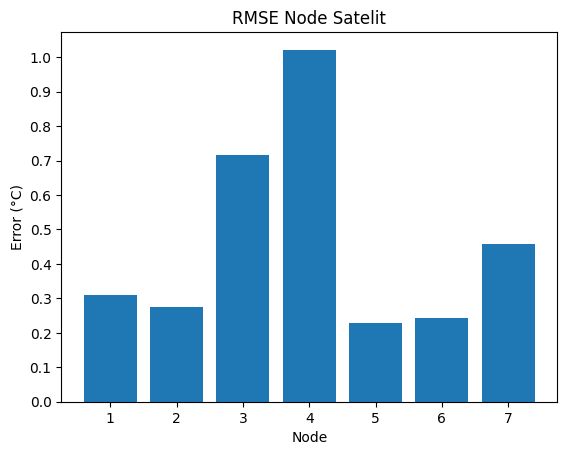
\includegraphics[width=0.6\textwidth]{figure/rmse_2018-05-20.png}
      \end{figure}
  \end{columns}
\end{frame}
\begin{frame}
  \frametitle{Hasil Pemodelan Termal Satelit LAPAN-A3}
  \begin{itemize}
    \item Secara kualitatif, model termal dapat menangkap tren dan nilai perubahan suhu \textit{node-node} satelit
    \item Secara kuantitatif, 5 dari 7 \textit{node} satelit menghasilkan skor $R^2$ lebih besar dari 0.95 dan 6 dari 7 \textit{node} memiliki nilai RMSE lebih kecil dari 1 $^\circ$C
    \item Artinya, model termal dapat memprediksi lebih dari 95\% tren perubahan suhu pada 5 \textit{node} dan memiliki rata-rata deviasi standar kesalahan prediksi suhu di bawah 1 $^\circ$C untuk 6 \textit{node}
    \item Skor $R^2$ paling rendah dimiliki \textit{node} 3 dan disusul oleh \textit{node} 7
    \item Nilai RMSE maksimum dimiliki \textit{node} 4 dengan nilai 1 $^\circ$C
  \end{itemize}
\end{frame}

\begin{frame}
  \frametitle{Analisis Penyebab Ketidakakuratan Model Termal}
  \begin{columns}[T]
    \column{0.5\textwidth}
      \begin{figure}
          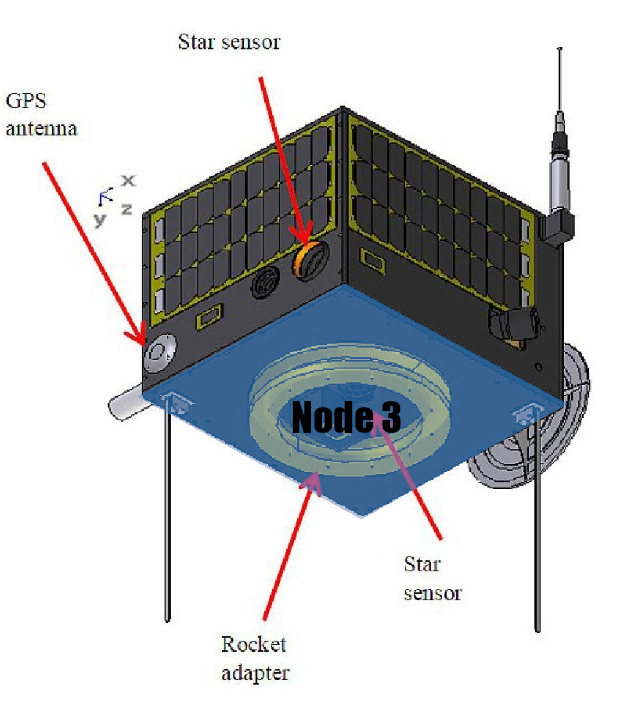
\includegraphics[width=0.5\textwidth]{figure/node3.png}
            \caption{Ilustrasi letak \textit{node} 3}
      \end{figure}
      \begin{figure}
          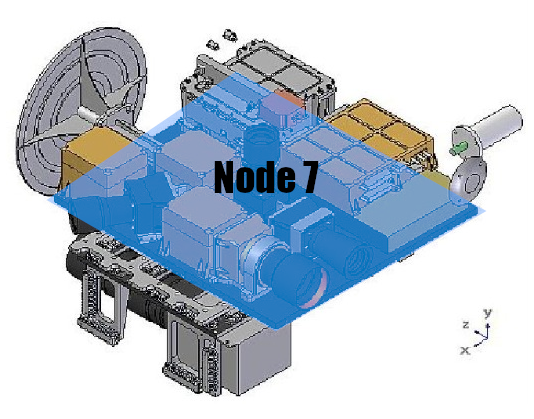
\includegraphics[width=0.5\textwidth]{figure/node7.png}
            \caption{Ilustrasi letak \textit{node} 7}
      \end{figure}
    \column{0.5\textwidth}
    \begin{block}{\center \normalsize Kapasitas termal rata-rata \textit{node}}
      \begin{itemize}
        \item Satelit LAPAN-A3 dimodelkan menjadi 7 titik analisis diskrit (textit{node})
      \item \textit{Node} yang terdiri dari komponen dengan material berbeda dapat memiliki rentang nilai kapasitas termal yang besar
      \item Rentang kapasitas termal besar dapat menyebabkan perbedaan perubahan suhu antar komponen \textit{node}
      \item Akibatnya, bacaan sensor suhu satelit dapat berbeda dengan suhu komponen-komponen sebenarnya
      \item Pada \textit{node} 3 terdapat \textit{rocket adapter} dan \textit{separation ring} serta pada \textit{node} 7 tersimpan banyak komponen elektronik satelit
      \end{itemize}
    \end{block}
  \end{columns}
\end{frame}

\begin{frame}
  \frametitle{Analisis Penyebab Ketidakakuratan Model Termal}
  \begin{columns}[T]
    \column{0.49\textwidth}
    \begin{block}{\center Pengaruh perubahan suhu \textit{node} lain}
      \begin{itemize}
        \item Perubahan suhu suatu \textit{node} dipengaruhi oleh perubahan suhu \textit{node-node} lain karena adanya konduksi dan radiasi antar \textit{node}
        \item Diperlukan analisis lebih lanjut untuk menentukan suku pada persamaan termal satelit yang mungkin menghasilkan \textit{error} besar pada persamaan termal satelit
        \item Jika ditemukan bahwa perubahan suhu \textit{node} 4 didominasi oleh perubahan suhu \textit{node} 3 dan 7, penjelasan mengenai kapasitas termal rata-rata dapat dipakai
        \item Sebaliknya, jika berbeda, hasil analisis dapat digunakan untuk melihat suku mana yang harus dihitung lebih akurat untuk memperkecil kesalahan prediksi model
      \end{itemize}
    \end{block}
    \column{0.02\textwidth}
    \column{0.49\textwidth}
    \begin{block}{\center Asumsi bentuk satelit}
      \begin{itemize}
        \item Satelit diasumsikan berbentuk balok sehingga \textit{node-node} dianggap berbentuk plat persegi panjang dalam perhitungan \textit{view factor}
        \item Ada komponen satelit yang tidak berbentuk persegi panjang seperti antena dan kamera
      \end{itemize}
    \end{block}
  \end{columns}
\end{frame}

% Bab 5
\section{Bab 5 - Kesimpulan dan Saran}
\begin{frame}
  \frametitle{BAB V}
  \center \large KESIMPULAN DAN SARAN
\end{frame}
\begin{frame}
  \frametitle{Kesimpulan}
  \begin{itemize}
    \item Langkah-langkah pemodelan termal semi-empiris satelit menggunakan metode \textit{machine learning} sudah dijelaskan
    \item Algoritma pemodelan termal yang dapat memprediksi suhu sisi-sisi satelit LAPAN-A3 juga sudah berhasil diimplementasikan
    \item Secara umum, model termal LAPAN-A3 dapat memprediksi tren dan nilai perubahan suhu sisi-sisi satelit
    \item Untuk kedua periode observasi, prediksi 5 dari 7 \textit{node} satelit menghasilkan skor $R^2$ lebih besar dari 0.95 dan 6 dari 7 \textit{node} satelit menghasilkan nilai RMSE lebih kecil dari 1 $^\circ$C.
  \end{itemize}
\end{frame}

\begin{frame}
  \frametitle{Saran}
\begin{enumerate}
\item Menambah jumlah \textit{node} yang digunakan dalam pemodelan sehingga karakteristik termal satelit dapat termodelkan lebih menyeluruh
\item Mengubah asumsi yang digunakan pada \textit{node} satelit untuk memodelkan karakteristik \textit{node} satelit lebih akurat
\item Melakukan analisis lebih lanjut untuk menghitung kontribusi tiap variabel dalam persamaan termal satelit
\item Memperpanjang durasi periode observasi sehingga data masukan yang dapat digunakan juga bertambah
\item Menggunakan data dari periode observasi saat satelit melakukan maneuver agar model termal dapat mengakomodasi efek perubahan sikap satelit lebih baik
\end{enumerate}
\end{frame}


\setbeamercovered{transparent}
\begin{frame}
  \frametitle{Daftar Pustaka}
  \tiny
  \bibliography{IEEEabrv,ref}
\end{frame}

\setbeamercovered{transparent}
\begin{frame}
  \frametitle{Appendix A - Perhitungan View Factor Plat Persegi Panjang ke Bola}
  Nilai \textit{view factor} dari permukaan plat persegi panjang 1 ke permukaan
  bola 2 $F_{1,2}$ dapat dihitung berdasarkan persamaan berikut \cite{martinez2022a}:
\begin{equation}
	F_{1,2} = 
\begin{cases} 
	\frac{\cos{\gamma}}{h^2} & ,\;|\gamma| \leq \cos^{-1}\left(\frac{1}{h}\right) \\
	\frac{1}{\pi h^2} \left( \cos{\gamma}\cos^{-1}y - x\sin{\gamma}\sqrt{1-y^2} \right) + \frac{1}{\pi}\tan^{-1}\left( \frac{\sin{\gamma}\sqrt{1-y^2}}{x} \right) & ,\;|\gamma| > \cos^{-1}\left(\frac{1}{h}\right) \\
\end{cases}
\label{eq:vf}
\end{equation}

  \begin{columns}[T]
    \column{0.5\textwidth}
    \begin{figure}
      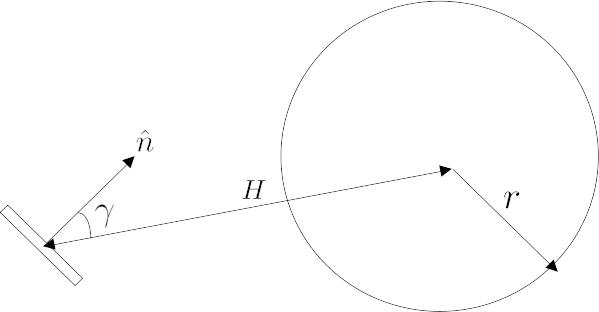
\includegraphics[width=0.8\textwidth]{figure/platball.png}
    \end{figure}
    \column{0.5\textwidth}
    \small
    \center Keterangan
    \begin{description}
      \item{$r$} Jari-jari bola
      \item{$\hat{n}$} Vektor normal permukaan plat
      \item{$H$} Garis jarak antara permukaan plat dan bola
      \item{$\gamma$} Sudut antara $\hat{n}$ dan $H$ 
      \item{$h$} $\frac{H}{r}$
      \item{$x$} $\sqrt{h^2 - 1}$
      \item{$y$} $-x \cot{\gamma}$
    \end{description}
  \end{columns}
\end{frame}

\setbeamercovered{transparent}
\begin{frame}
  \frametitle{Appendix B - Grafik Sikap Satelit LAPAN-A3 vs Waktu}
  \begin{columns}[T]
    \column{0.5\textwidth}
    \center 19 Mei 2018
      \begin{figure}
          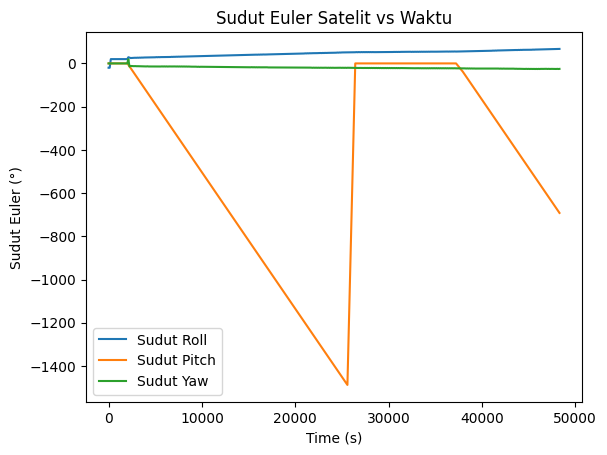
\includegraphics[width=0.8\textwidth]{figure/attitude_2018-05-19.png}
      \end{figure}
    \column{0.5\textwidth}
    \center 20 Mei 2018
      \begin{figure}
          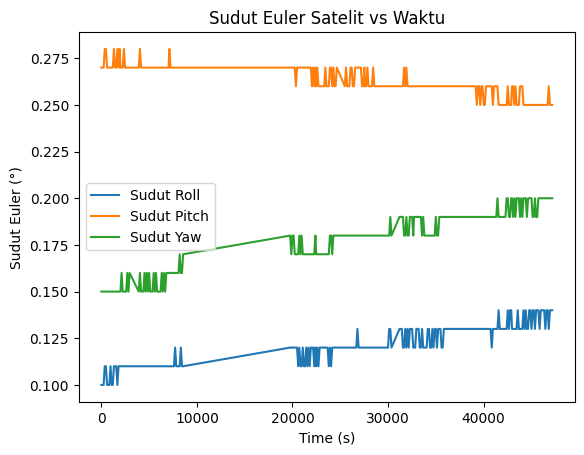
\includegraphics[width=0.8\textwidth]{figure/attitude_2018-05-20.png}
      \end{figure}
  \end{columns}
\end{frame}

\setbeamercovered{transparent}
\begin{frame}
  \frametitle{Appendix C - Orbit \textit{Sun-synchronous}}
  \begin{columns}[T]
    \column{0.5\textwidth}
    \begin{block}{Ilustrasi orbit \textit{sun-synchronous}}
      \begin{figure}
          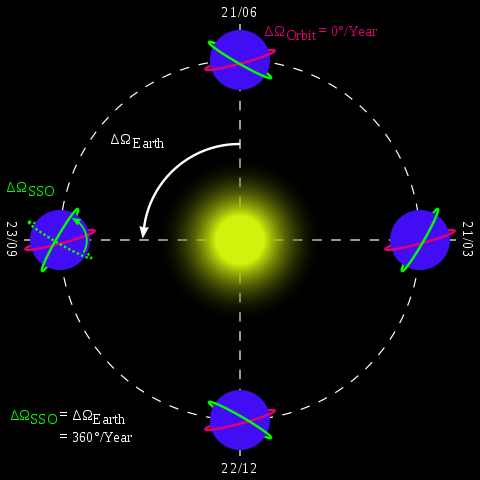
\includegraphics[width=0.8\textwidth]{figure/sso.png}
      \end{figure}
      Orbit \textit{sun-synchronous} ditunjukkan orbit dengan warna hijau
    \end{block}
    \column{0.5\textwidth}
    \begin{itemize}
      \item Orbit \textit{sun-synchronous} memiliki sudut antara vektor normal orbit satelit dengan vektor arah Matahari-Bumi yang konstan sepanjang tahun
      \item Satelit akan cenderung mendapatkan pencahayaan yang konsisten sepanjang tahun
      \item Satelit juga akan melintasi khatulistiwa Bumi pada waktu lokal yang relatif sama setiap hari (pukul 09.30 untuk LAPAN-A3 di \textit{ground station} LAPAN, Bogor)
    \end{itemize}
  \end{columns}
\end{frame}

\setbeamercovered{transparent}
\begin{frame}
  \frametitle{Appendix D - Regresi Linear}
  \begin{columns}[T]
    \column{0.4\textwidth}
    \begin{itemize}
      \item Pendekatan untuk memodelkan hubungan antara variabel dependen dan variabel independen secara linear
      \item Model regresi linear akan menghitung matriks $w$ yang memetakan matriks $X$ ke $Y$ dan meminimalkan matriks $\varepsilon$ 
    \end{itemize}
    \column{0.6\textwidth}
    \begin{equation}
      \label{eq:reglinear}
      Y = Xw + \varepsilon
    \end{equation}
    \center Keterangan
    \begin{description}
      \item{$Y$} Matriks variabel dependen
      \item{$X$} Matriks variabel independen
      \item{$w$} Matriks koefisien yang tidak diketahui
      \item{$\varepsilon$} Matriks kesalahan atau gangguan
    \end{description}
  \end{columns}
\end{frame}

\setbeamercovered{transparent}
\begin{frame}
  \frametitle{Appendix E - Maneuver Khusus LAPAN-A3}
  \begin{columns}[T]
    \column{0.49\textwidth}
    \begin{block}{Maneuver \textit{stop and release with roll}}
      \begin{figure}
          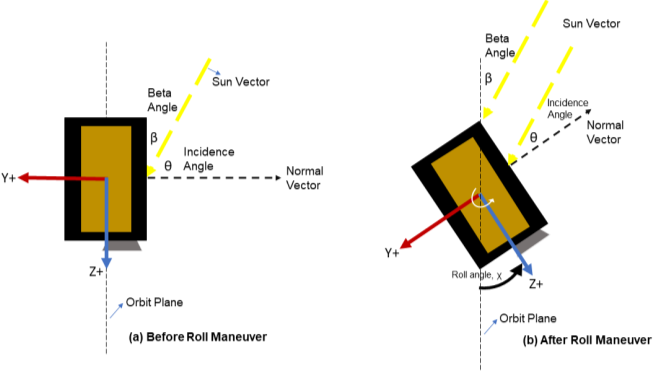
\includegraphics[width=0.8\textwidth]{figure/maneuver2.png}
      \end{figure}
      \begin{figure}
          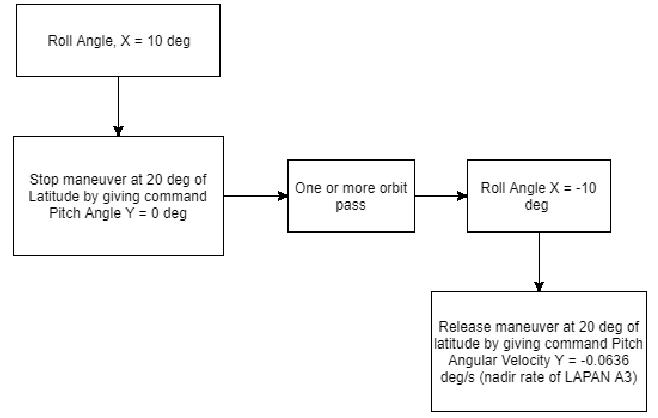
\includegraphics[width=0.8\textwidth]{figure/exmaneuver2.png}
      \end{figure}
    \end{block}
    \column{0.02\textwidth}
    \column{0.49\textwidth}
    \begin{block}{Maneuver \textit{stop and release}}
      \begin{figure}
          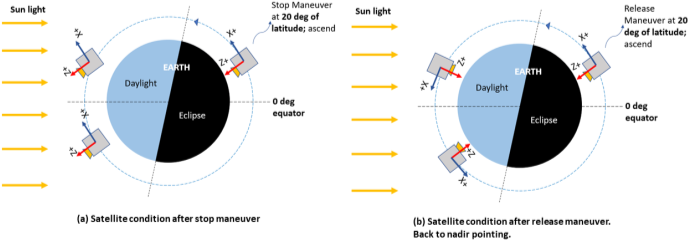
\includegraphics[width=0.8\textwidth]{figure/maneuver1.png}
      \end{figure}
      \begin{figure}
          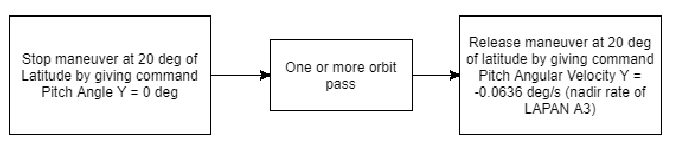
\includegraphics[width=0.8\textwidth]{figure/exmaneuver1.png}
      \end{figure}
    \end{block}
  \end{columns}
\end{frame}


\end{document}
